\subsection{Lock-free структуры данных}
\label{lockfree:section}
	
В многопоточных программах проблемы при совместной работе потоков обычно возникают при доступе к общим ресурсам.
Помимо блокирующего подхода, использующего примитивы синхронизации, также используется неблокирующий подход.
Для того, чтобы избежать состояния гонки можно использовать специальные неблокирующие структуры данных.
Данный подход основывается на использовании атомарных переменных и lock-free или wait-free объектов.
	
Разделяемый объект называется lock-free объектом, если он гарантирует, что некоторый поток закончит выполнение операции над объектом за конечное число шагов вне зависимости от результатов работы других потоков.
	
Объект является wait-free, если каждый поток завершит операцию над объектом за конечное число шагов.
	
Может возникнуть вопрос, зачем нужны неблокирующие структуры данных, если можно использовать примитивы синхронизации для доступа к обычной структуре данных.
Lock-free структуры имеют ряд преимуществ над блокирующими структурами данных.
Так, по пропускной способности они превосходят блокирующие в 1.5--3 раза, однако как блокирующие, так и неблокирующие очереди имеют слабую масштабируемость относительно числа потоков.
По величине задержки элементов в очереди неблокирующие очереди также имеют лучшие характеристики, однако их преимущество достаточно мало.
Также использование примитивов синхронизации может привести к deadlock, а также могут возникать ошибки, связанные с забыванием захвата или освобождения примитивов.
	
Lock-free структуры данных не содержат блокировок и остаются в консистентном состоянии вне зависимости от числа потоков, одновременно обращающихся к ней.
Такие структуры данных можно организовать с помощью RMW (read-modify-write) -- операции чтения, изменения и записи, происходящая атомарно.
	
Примером RMW операции может служить CAS. В библиотеке C++ существует два варианта реализации этой операции: weak и strong.
Weak версия может вернуть false в случае, когда считанное значение было равно ожидаемому.
Strong всегда возвращает правильное значение.

\begin{minted}{c++}
bool compare_exchange_weak(T& expected, T desired, 
                           std::memory_order success, 
                           std::memory_order failure) noexcept;

bool compare_exchange_strong(T& expected, T desired, 
                             std::memory_order success, 
                             std::memory_order failure) noexcept;
\end{minted}

Альтернативой CAS операций служит пара LL/SC операций в ARM процессорах.
Load-link операция загружает значение из памяти, а store-conditional устанавливает новое значение, но только в том случае, если область памяти не менялась.
Для реализации LL/SC операций пришлось изменить структуру кэша: к каждой линии кэша добавляется флаг LINK. Флаг устанавливается при операции LL и сбрасывается при SC или вытеснении кэш-линии.
LL/SC операции не подвержены проблеме ABA, однако из-за аппаратной реализации может возникать false sharing.
В современных процессорах длина кэш-линии составляет 64--128 байт, следовательно, в одной кэш-линии может находиться несколько переменных.
При работе с несколькими переменными в одной линии у LL/SC операций будет общий флаг LINK, что может привести к неправильной работе.
Чтобы данной проблемы не возникало, следует размещать по одной переменной в линии.

\inputminted{c++}{listings/falseSharingLLSCExample.cpp}

CAS операцию можно достаточно легко реализовать с помощью LL/SC операций:

\inputminted{c++}{listings/LLSCthroughCAS.cpp}

Также важно понимать, что lock-free алгоритмы чувствительны к переупорядочению машинных инструкций в их коде.
Чтобы избежать этого используются барьеры памяти.
Барьер памяти X\_Y гарантирует, что все X-операции до барьера будут выполнены до того как начнут выполняться Y-операции после барьера.
В теории существует 4 вида барьеров -- LoadLoad, LoadStore, StoreLoad, StoreStore, однако не все из них реализованы по всех архитектурах.
Существует 4 модели памяти процессоров:
	
\begin{itemize}  
    \item\textbf{Relaxed model} -- возможно переупорядочение любых инструкций обращения к памяти, даже зависящих по данным (DEC Alpha).
    \item\textbf{Weak model} -- возможно переупорядочение любых инструкций чтения и записи, кроме тех, которые имеют зависимости по данным (ARM, PowerPC, Intel Itanium).
    \item\textbf{Strong model} -- возможно только переупорядочение вида чтение до записи (x86).
    \item\textbf{Sequentual consistency model} -- любое переупорядочение запрещено.
\end{itemize}

Существуют различные lock-free структуры данных: очереди (со строгим и ослабленным порядком), стек, связные списки, хеш-таблицы.
В C++ данные структуры данных можно использовать подключая различные библиотеки.
Например, Boost содержит реализацию очереди и стека, а Libcds -- все перечисленные.

Примером lock-free структуры данных может служить очередь Майкла-Скотта.
Эта очередь реализуется на базе односвязного списка и двух указателей, один из которых указывает на голову списка (dummy node), а другой -- на хвост (рисунок~\ref{lockFreeQueue:image}).

\begin{figure}[H]
    \centering
    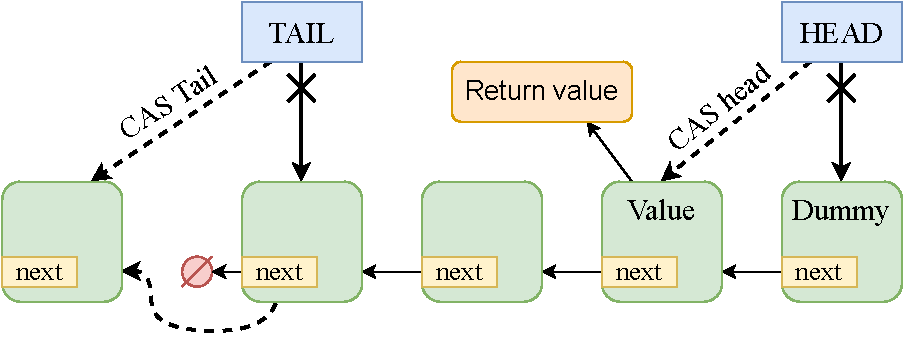
\includegraphics[width=\linewidth]{lock_free_queue}
    \caption{Очередь Майкла - Скотта}
    \label{lockFreeQueue:image}
\end{figure}
	
Рассмотрим упрощенный код очереди из библиотеки libcds.
Ниже представлена функция enqueue -- добавления в очередь.
Сначала переданное значение кладется в node.
Затем мы пытаемся положить его в хвост очереди.
После получения текущего хвоста указатель продвигается, пока не дойдет до фактического хвоста.
Затем значение ставится в конец очереди, и хвосту присваивается значение вставленного элемента.

\inputminted{c++}{listings/lockFreeQueueEnqueue.cpp}
	
Для того чтобы достать элемент из очереди (функция dequeue), необходимо, чтобы очередь не была пуста, а также чтобы хвост и голоса были продвинуты.

% TODO: Начать нумеровать листинги?
Код функции приведен ниже.
\inputminted{c++}{listings/lockFreeQueueDequeue.cpp}

